\documentclass[12pt,a4paper]{report}
\usepackage[utf8]{inputenc}
\usepackage[english]{babel}
\usepackage[T1]{fontenc}
\usepackage{geometry}
\usepackage{setspace}
\usepackage{graphicx}
\usepackage{hyperref}
\usepackage{listings}
\usepackage{xcolor}
\usepackage{float}
\usepackage{caption}
\usepackage{subcaption}

\geometry{left=3cm, right=2cm, top=2.5cm, bottom=2.5cm}
\onehalfspacing

\hypersetup{
    colorlinks=true,
    linkcolor=black,
    filecolor=magenta,      
    urlcolor=blue,
    citecolor=black
}

\lstset{
    basicstyle=\ttfamily\small,
    keywordstyle=\color{blue},
    commentstyle=\color{green!60!black},
    stringstyle=\color{red},
    showstringspaces=false,
    breaklines=true,
    frame=single,
    backgroundcolor=\color{gray!10}
}

\begin{document}

\begin{titlepage}
    \centering
    {\Large \textbf{"ALEXANDRU IOAN CUZA" UNIVERSITY OF IAȘI}}\\[0.5cm]
    {\Large \textbf{FACULTY OF COMPUTER SCIENCE}}\\[2cm]
    
    \begin{center}
    
\includegraphics[width=0.3\textwidth]{images/logoFii.png}
    \end{center}

    {\Huge \textbf{Bachelor's Thesis}}\\[1cm]
    {\Huge \textbf{Off Course - Web Platform for Exploring Abandoned Buildings in Romania}}\\[3cm]

    {\Large proposed by}\\[1cm]

    {\Large Popa Cosmin-George}\\[2cm]
    
    {\large Session: July, 2025}\\[1cm]
    
    {\large Scientific Coordinator}\\
    {\large Lect. Univ. Dr. Pătruț Bogdan}\\[2cm]
    
    \vfill
\end{titlepage}

\newpage
\begin{center}
{\Large \textbf{"ALEXANDRU IOAN CUZA" UNIVERSITY OF IAȘI}}\\[0.5cm]
{\Large \textbf{FACULTY OF COMPUTER SCIENCE}}\\[3cm]

{\Large \textbf{Off Course - Web Platform for Exploring Abandoned Buildings in Romania}}\\[3cm]

{\Large \textbf{Popa Cosmin-George}}\\[2cm]

{\large Session: July, 2025}\\[2cm]

{\large Scientific Supervisor}\\
{\large \textbf{Prof. Dr. Pătruț Bogdan}}\\[2cm]
\end{center}

\textbf{Off Course - Web Platform for Exploring Abandoned Buildings in Romania}

\newpage

\chapter*{Declaration of Originality}
\addcontentsline{toc}{chapter}{Declaration of Originality}

I, Popa Cosmin-George, domiciled in strada Mihai Eminescu nr.51 Galați, born on 01.03.2003, identified by CNP 5030301170011, graduate of Alexandru Ioan Cuza University of Iași, Faculty of Computer Science, specialization Computer Science in English, class of 2025, declare on my own responsibility, knowing the consequences of false statements under art. 326 of the New Penal Code and the provisions of the National Education Law no. 1/2011 art.143 par. 4 and 5 regarding plagiarism, that the bachelor's thesis entitled:

\textbf{Off Course - Web Platform for Exploring Abandoned Buildings in Romania}

developed under the guidance of Lect. Univ. Dr. Pătruț Bogdan, which I will present before the commission is original, belongs to me and I assume full responsibility for its content.

I also declare that I agree that my bachelor's thesis may be verified by any legal means to confirm its originality, including consenting to the introduction of its content into a database for this purpose.

I have been informed that the commercialization of scientific papers in order to facilitate falsification by the buyer of the quality of author of a bachelor's thesis, diploma or dissertation is prohibited, and in this regard, I declare on my own responsibility that the present work has not been copied but represents the result of the research I have undertaken.

\vspace{2cm}
Date: \hfill Student signature

\newpage

\chapter*{Declaration of Consent}
\addcontentsline{toc}{chapter}{Declaration of Consent}

I hereby declare that I agree that the Bachelor's thesis entitled "Off Course - Web Platform for Exploring Abandoned Buildings in Romania", the source code of the programs and other contents (graphics, multimedia, test data, etc.) that accompany this work may be used within the Faculty of Computer Science.

I also agree that the Faculty of Computer Science at Alexandru Ioan Cuza University of Iași may use, modify, reproduce and distribute for non-commercial purposes the computer programs, in executable and source format, developed by me as part of this bachelor's thesis.

\vspace{2cm}
Iași, \hfill Graduate Popa Cosmin-George


\tableofcontents
\newpage

\chapter*{Abstract}
\addcontentsline{toc}{chapter}{Abstract}

Off Course is a new way to think about urban exploration. The website provides a map with a rich selection of abandoned buildings, waiting to be photographed and a gamified way to document them.

The application is built using Node.js with the Express framework for its backend, basic HTML and CSS for the frontend (Leaflet for the map UI) and MongoDB as the database system. In terms of security, JWT is used for authentication, along bcrypt that ensures data secrecy via hashing. The platform's main way of adding new locations is the Google Places API.

The research put into creating this project is based on the already existing similar services and figuring out their weaknesses in terms of user satisfaction. The solution I am presenting is one that is specifically for the country of Romania and includes extra features like the game-like system. As well as that, real data is provided to me by a community I am part of.

Testing results highlight that the website is functional for multiple users at the same time, with a low response time and clean look for both desktop and mobile.

\newpage

\chapter*{Introduction}
\addcontentsline{toc}{chapter}{Introduction}

\section*{Motivation for Topic Selection}

Urban exploration, also known as "urbex" online is the practice of taking pictures of abandoned buildings, usually in urban areas, for artistic or documentation purposes. In Romania, there is an abudance of these types of places, but no thorough "compendium" exists as of yet.

The motivation for developing the platform was born from the voices in the community that needed an easily accessible, yet secure resource. Information about places of interest is scattered all over the internet, on forums(subreddits), other similar applications or close-knit communities.

Below is the poster for an art exhibition about forgotten buildings, created by Victor Ioan, an individual that is part of my Urbex community on Discord.

\begin{center}

\includegraphics[width=0.4\textwidth]{images/expozitie.jpg}
\end{center}

As apparent from the message below, he is dissatisfied with the current applications on the market, not just about the number of spots that are listed, but also about the details regarding accessing them physically.

\begin{center}

\includegraphics[width=0.8\textwidth]{images/mesaj.png}
\end{center}

The use of web technologies, mainly Node.js, highlights the characteristics of a modern, scalable and maintainable solution for all enthusiasts. Alongside it, the integration of the interactive way of "exploring" is innovative and unique.



\section*{Problem Statement}

The Romanian urban exploration community has to deal with the following challenges:

\begin{itemize}
    \item \textbf{Spread Information}: Location data is unfocused, ranging from forums, applications, websites and other forms of online groups; as well as few and far between, meaning  
    
    \item \textbf{Quality and Safety}: A rating system does not exist for hobbyists to tell whether a location is safe, accessible or worth visiting
    
    \item \textbf{Accessibility}: A map with most, if not all possible locations does not exist for the country of Romania
    
    \item \textbf{Community}: The gamification elements could determine more people to discover and get into the hobby of urban exploration 
\end{itemize}

These challenges collectively result in a far from perfect experience for the existing and growing community of urbex in Romania.

\section*{Research Objectives}

\subsection*{Primary Objectives}

The objective of this research is to design and implement a web platform that caters as a hub for all romanians passionate about urban exploration. This involves:

\begin{enumerate}
    \item \textbf{Development of a Modern Web Application}: Creating a full-stack application using powerful technologies that ensure a nice and intuitive experience for users (desktop and mobile).
    
    \item \textbf{Implementation of an Advanced Map}: Combining Google Maps API with Leaflet for a precise visualisation and discovery mechanism for abandoned buildings.
    
    \item \textbf{Robust Security}: Guaranteed security is achieved by the implementation of JWT for user sessions, logging in and validation. bcrypt ensures a safe way of storing sensitive information like passwords.
    
    \item \textbf{Gamification System}: Unique user engagement provided by the leveling up system via experience points and leaderboard for both participants and abandoned spots.
\end{enumerate}

\subsection*{Secondary Objectives}

Other objectives that enhance the platform's priorities are:

\begin{enumerate}
    \item \textbf{Community Quality}: Implementing an invite-only registration system(like filelist) to share critical data about these spots to only trusted individuals.
    
    \item \textbf{Reduced-Cost Deployment}: Demonstrating the capability of hosting the platform on and affordable hardware peice like the Raspberry Pi Zero 2.
    
    \item \textbf{Scalability and Maintainability}: By using an optimised MVC architecture, future improvements and user input data can easily be tackled.

\end{enumerate}

\section*{Methodology Overview}

The development methodology applied to this project involves strategies learnt at various subjects at the Faculty of Computer Science, like Web Technologies, Software Engineering, Advanced Topics in .NET, Information Security, Data Bases and DBMS Practice.

\textbf{Research Phase}: In-depth analysis of already existing similar platforms like Urbexology, Abandoned World and r/UrbexRo, with the sole purpose of identifying what gaps there are to fill with this project.

\textbf{Evaluation of Technology}: Comparison of the available technologies for building such a project, in terms of the programming language, database solution, frameworks and architecture.

\textbf{Prototype Development}: Developing and testing each feature, one by one, in order to ensure a satisfactory functionality for end users.

\textbf{Security Implementation}: Understanding the importance of security measures that needed to be adopted, like JWT, bcrypt and CORS.

\textbf{Testing}: Checking to see if the solution is as close to the desired result as possible in terms of backend, API endpoints and user interface.

\section*{Solution Summary}

Off Course is the solution that fixes the identified issues specified above by using modern web technologies and a clean design. The three main layers of the application are:

\textbf{Frontend Layer}: Built with vanilla JavaScript, HTML5, and CSS3, being complemented by Leaflet for an interactive mapping. The interface is intuitive and is responsive for mobile devices.

\textbf{Backend Layer}: Implemented using Node.js and the Express.js framework, incorporating popular libraries including bcrypt for hashing, multer for uploading files, jsonwebtoken for authentication, and CORS for cross-origin requests. Configuration is made privately in a .env file with all of the hidden variables.

\textbf{Data Layer}: MongoDB is a very flexible JSON based storage for data and is perfect for working with geographic data and user related content.

\textbf{*}The gamification model is incentivising for users to interact with because of the experience points gained after posting pictures and reviews.

\section*{Thesis Structure}

The thesis is organized into six chapters that describe the lifecycle of the whole development process:

\begin{itemize}
    \item \textbf{Chapter 1}: Highlightes the problem that exists and puts into context the need for a Romanian urban exploration platform.
    
    \item \textbf{Chapter 2}: Analyzes and compares already existing solutions and considers the design strategies.
    
    \item \textbf{Chapter 3}: Details requirements analysis and system design, including functional
and non-functional requirements with specic focus on the complete technology
stack. TO CHANGE LATER
    
    \item \textbf{Chapter 4}: Implementation documentation including all libraries (JWT, bcrypt, CORS, multer, dotenv, Axios, Leaflet).
    
    \item \textbf{Chapter 5}: Presents testing and validation for the platform, by me and a friend.
    
    \item \textbf{Chapter 6}: Views the deployment process on the Raspberry Pi Zero 2.
\end{itemize}

The conclusions will give a succint overview of the state of the project, if the goals have been achieved and what to look for in the future in terms of development.

\section*{Expected Contributions}

This research contributes to the academic field of web application development, as well as the practical needs of the urban exploration community in Romania:

\textbf{Technical Contributions}:
\begin{itemize}
    \item Demonstration of effective integration between two different double mapping technologies (Google Maps API and Leaflet)
    \item Implementation case study for gamification in niche community platforms
    \item Security best practices documentation for community-driven applications
    \item Techniques for optimising applications with a multitude of media (images).
\end{itemize}

\textbf{Community Contributions}:
\begin{itemize}
    \item The first centralised platform designed for Romanian urban exploration
    \item Quality-controlled environment for sharing location information and safety data
    \item A way for the existing community to grow in the future
    \item Open source code will be posted on github for adaptation or improvements.
\end{itemize}

\newpage

\chapter*{Personal Contributions}
\addcontentsline{toc}{chapter}{Personal Contributions}

The main contributions of this work include:

\begin{itemize}
    \item Development of a web platform specifically designed for the Romanian urban exploration community
    \item Implementation of an interesting gamification system that encourages user to participate actively
    \item Integration of multiple mapping technologies (Google Maps API with Leaflet) for best results in terms of discovery
    \item Maintaing a secure invite-only way of access to ensure only those passionate enough can join
    \item Implementing a scalable architecture that can be deployed on a cheap Raspberry Pi
    \item Industry standard security is provided for all users, because their data is important
    \item Developing an efficient way of uploading files via Multer for the pictures
    \item Using a RESTful API that is best practice for all application by today's standards
\end{itemize}

\newpage

\chapter{Problem Description}
\section{Context of Urban Exploration in Romania}
Urban Exploration is a term not known by many, but slowly gaining popularity in recent years, with the "mainstreamification" of vlogs, social media and personal websites.

The general definition is: "Urban exploration (often shortened as urbex) is the exploration of manmade structures, usually abandoned ruins or hidden components of the manmade environment. Photography and historical interest/documentation are heavily featured in the hobby."~\cite{wikipediaUrbexDefinition}.

In Romania, this practice is more obscure, but still appreciated, as seen from an article: "Există iubitori ai explorărilor de acest gen şi în România. Fiind o activitate complet de nişă, munca acestori oameni trece neobservată de cele mai multe ori, cu toate că rezultatele sunt de-a dreptul uimitoare./There are enthusiasts of this kind of exploration in Romania as well. Being a completely niche activity, the work of these people often goes unnoticed, even though the results are truly astonishing."~\cite{articleUrbexRomania}

\section{Identified Problems}
\subsection{Information Fragmentation}
Information about locations, meaning coordinates or general description are definitely not centralized. Info about spots is being kept secret or just simply not shared even though it could prove useful to responsible enthusiasts, as stated by "Liviu Stan, explorator urban: „E o competiție în zona asta, cine este primul acolo își înfige steagul și nu vrea să dea mai departe./Liviu Stan, urban explorer: "It's a competition in this area, whoever gets there first plants their flag and doesn't want to share it with anyone else."~\cite{articleUrbexInformation}

\subsection{Discovery Challenges}
Another main obstacle when wishing to document these types of places could be actually finding them in the first place. These spaces are more often than not hidden, sealed and also concealed digitally, having to hear about them through word-of-mouth.

The platform aims to solve this by giving everyone an intuitive, easy and clean map interface to view all locations.

\subsection{Safety and Quality Issues}
To no one's surprise, documenting old abandoned buildings is by no means a safe or easy feat. Evidently, the more is known about a location beforehand, the safer it is for other people to visit it later and that is why it is of high importance that details about the quality of such spots is available: "Cristian Lipovan, explorator urban, fotograf: La fața locului, tot timpul mă asigur să nu cadă ceva, să nu fie o chestie care poate să se rupă, să cadă, e foarte important să respectăm locul în care intrăm, să nu distrugem nimic/Cristian Lipovan, urban explorer, photographer: On site, I always make sure nothing is about to fall, that there's nothing that could break or collapse, it's very important to respect the place we're entering and to not destroy anything."~\cite{articleUrbexInformation}

\subsection{Community Fragmentation}
The community of urbex enjoyers is quite separated, seeing as it is not a very social sport. Such an ambitious platform could help more of them to connect with eachother, as it would certainly be a common interest/talking point.

\section{Target Audience Analysis}
\subsection{Users' characteristics}
The types of people that would be interested in using the platform are:
\begin{enumerate}
    \item urban exploration enthusiasts
    \item professional or amateur photographers
    \item history or architecture lovers
    \item tourists looking for a different experience
\end{enumerate}

Even though these backgrounds are diverse, each of them share common characteristics, those being they are young adults, between 18-35 years of age, digitally educated and generally respectful and curious by nature.

\subsection{Invite Criteria}
As with any other activity, though, a vocal minority can ruin the reputation and enjoyment for the people actually passionate about this sport. Off Course is aware that not everybody wanting to access its resources may have the best intentions in mind, hence invitations will be sent personally to users that can prove their methods are not destructive.

"În comunitatea aceasta există şi o 'lege' care spune că exploratorii urbani nu trebuie niciodată să ia ceva din locurile pe care le fotografiază, cu excepţia imaginilor./In this community, there is also an 'unwritten rule' that urban explorers must never take anything from the places they photograph, except for images."~\cite{articleUrbexRomania}

There have been numerous controversies in the media because of irresponsible people that find out about these locations via publicly available resources, like Reddit, issue that Off Course wants to avoid."polițiștii din Capitală au dat trei amenzi, în valoare totală de 800 de lei, după ce au prins un grup de 18 adolescenți cățărați pe o clădire din centru./police in the capital issued three fines totaling 800 lei after catching a group of 18 teenagers climbing on a building in the city center."~\cite{articleUrbexControversy} Ever since then, the reddit community's rules do not allow users to post location details anymore.

\chapter{Related Work and Existing Solutions}
\section{International Applications Analysis}
\subsection{Abandoned World}
The most popular similar platform is a smartphone app called Abandoned World.

According to their App Store description, it reaches numbers like: "700,000+ active explorers" and "250,000+ locations worldwide"~\cite{appAbandonedWorld}

\begin{center}
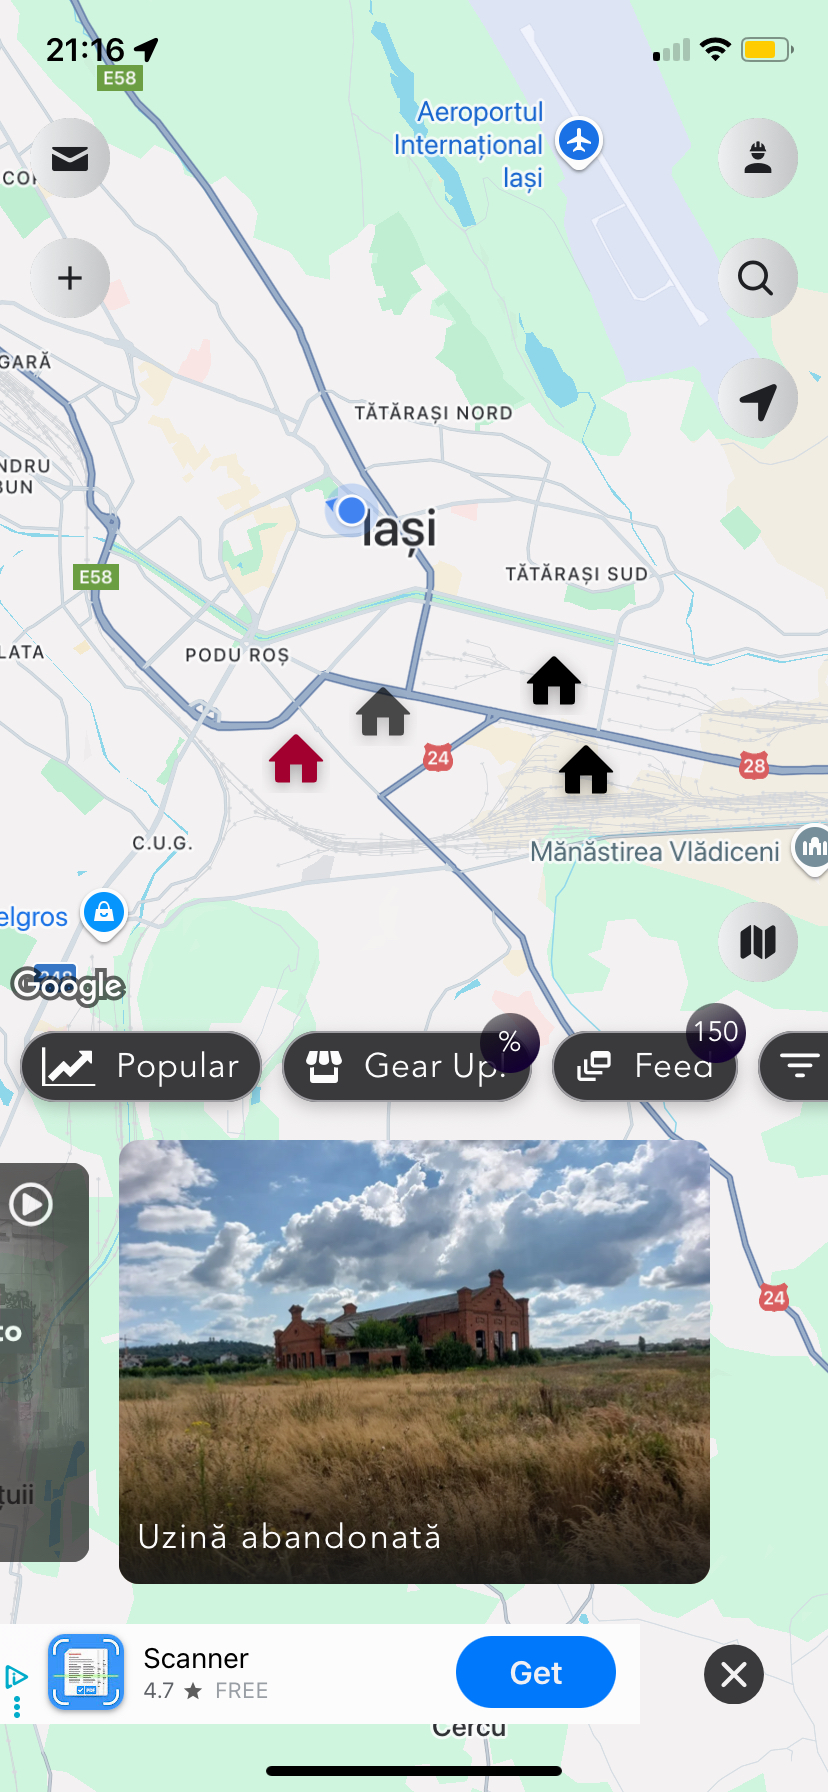
\includegraphics[width=0.3\textwidth]{images/abandonedworld.png}
\end{center}

The app is clean looking and shares a lot of features with Off Course, however, being an international project, not a lot of locations are available specifically for Romania. All locations are submitted by users and are not validated correctly and there is no use of the Google Places API in order to obtain more spots automatically.
As well as that, there is no incentive to see the locations for yourself, as no reward system exists. 

\subsection{Urbexology}
A bit under the radar, yet more used in Romania is Urbexology.

"This website is intended solely for informational, archival, and artistic purposes. The locations presented on Urbexology are collected from publicly available sources, historical records, and community-contributed materials"~\cite{appUrbexology}

\begin{center}
\includegraphics[width=0.8\textwidth]{images/urbexology.png}
\end{center}

In terms of romanian locations, it performs much better than the mobile app alternative, however, again, there is no automation in terms of adding locations to the map via Google. A level up system does exist, but it is more limited, in the sense that you level up by submitting locations, but not exploring them yourself, meaning people would feel less motivated to go to existing locations and add pictures or detailed descriptions.

\section{Technology Stack Analysis}
\subsection{Mapping Solutions Comparison}

The mapping technology is obviously very important since it is the core of a platform such as this one. There are many options out there for embedding a functioning map to a website, the main ones being Google Maps and Leaflet with OpenStreetMap.

Google Maps is the top player, being controlled by a tech behemoth, with the best and most varied location data in the world. But, there is always a downside. Using Google Maps' services becomes expensive after repeated usage and, on top of that, customisability is limited.

After looking at both, I chose to combine the both of them, in order to get very accurate locations from Google Maps and, at the same time, a nice looking map UI for the user.

\subsection{Backend Technologies Evaluation}
When looking at the backend technology, the choice was much easier, since I am familiar with creating a web application because of a course from the faculty of computer science. 

Node.js is something that was used on a previous project and it is extremely capable, yet not overcomplicated. On top of that, Express is perfect for creating websites as it simplifies the development process.

MongoDB was picked as opposed to any other database because of its flexbility in terms of storing data. It is much easier to work with JSON-like records instead of fields in tables. This proved very useful in the process of creating the application because necessary fields that were not added at first were added on the way.

\section{Gap Analysis}
After this much research on the topic, it is clear that existing similar platforms do not provide nearly enough content for users, neither do they present details like access information or safety head-up's. 

What Off Course wants to further add new in terms of the urbex market is the game-like system and the Google Places API automation.

For this platform to be successful in terms of data, some matter of time will need to pass since it is built mainly on user suggestions, feedback and information but I believe, with time, it will be possible with a smaller, yet dedicated fan base, since it will basically tackle most issues of the user generated content models:"User-generated content (UGC) has the potential to be diverse and authentic, but it also comes with challenges related to its accuracy, relevance, and professionalism. Since UGC is created by individuals who may have a different level of expertise or understanding than the brand, there can be variations in the quality of content produced."~\cite{ugcChallenges}


\chapter{Requirements Analysis and System Design}
\section{Functional Requirements}
\subsection{User Management}
When connecting to the website, a user is required to sign up or log in to an account, otherwise, no information will be accessible (other than the about us page, of course).

After being prompted to log in, the user information is saved to the database according to the model. 

\begin{center}
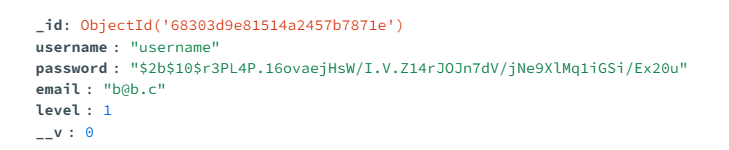
\includegraphics[width=1\textwidth]{images/user db.png}
\end{center}

As obvious from the example image, users' sensitive data is hashed for privacy and only required data is collected. As well as that, by using MongoDB, each creation request can be completed.

After creating a user record, each customer can view their profile with information about them and what they have achieved on the platform, as well as have access to all of the basic operations, like logging out, viewing locations and leaderboards and sending requests.

*It is important to mention that as the platform grows in numbers, an "admin" user feature should be implemented, in order to allow users to register or delete users that should be banned from accessing the service in the future.

\subsection{Location Management}
Locations are the most important feature of the platform, so it makes sense that a lot of information is stored about them in the database and also available to view when clicking on a spot's marker.

The two main sources of improving the website with more locations are the automatic search by Google Places API and the user submitted requests of trusted individuals, including myself and my friends.

Coordinates and other details will only be displayed for users to actually see after the request has been personally validated to make sure it is a real location and the descriptions are accurate. 

\subsection{Gamification System}
The gamification system is inspired by a lot of popular apps, games(Pokemon GO) or other types alike(Duolingo), that reward the user when completing tasks.

Experience points can be gained by visiting a location on the map, writing a review about a location you have visited and uploading relevant pictures. This helps the platform improve the quality of its content, but also make the players feel like they are actively participating and get rewarded for it.

After enough experience points are given to a player, his level increases, but the higher your level is, the more experience points you will need to level up.

This also creates a fun way to see who in the community is the most active via the leaderboard section and this can also determine people to meet other like-minded explorers and create new connections.

\subsection{Social Features}
The social features are, at the moment limited, but for a good reason. The platform will work very closely to the already existing dedicated Discord server, where a sense of community already exists. That is why I believe that adding social features to the application was not a priority.

\begin{center}

\includegraphics[width=0.5\textwidth]{images/discord.png}
\end{center}

\section{Non-Functional Requirements}
\subsection{Performance Requirements}
The website is not a service that requires a lot of processing power, neither on the client side, nor on the server side. Because the amount of locations that have to be loaded is not very high and also the amount of users will not go over the hundreds, the website is great in terms of performance.

This is convienient also for people that log onto it from their phone, since computers and laptops are faster, yet will be less used by the usual user.

\subsection{Security Requirements}
Security for the website is very strong thanks to the technologies that it makes use of.

-JWT is amazing for cookie sessions, retrieving relevant user data and redirecting people that should have no access from a specific page.
"JSON Web Token (JWT) defines a compact and self-contained way for securely transmitting information between parties as a JSON object. This information can be verified and trusted because it is digitally signed."~\cite{JWT}

-bcrypt hashes the users' passwords so their information remains private and impossible to break:
"bcrypt was designed based on the Blowfish cipher: b for Blowfish and crypt for the name of the hashing function used by the UNIX password system. [...] bcrypt forces you to follow security best practices as it requires a salt as part of the hashing process. Hashing combined with salts protects you against rainbow table attacks"~\cite{bcrypt}

-the invite system will ensure only people that have been invited can actually create an account and use the platform

\subsection{Usability Requirements}
The platform is modern so using it is very intuitive. It looks clean, with buttons that indicate what each of them does and tabs on the UI for going inbetween pages. The application is also responsive on mobile and it can also be easily used there.

\subsection{Scalability Requirements}
As mentioned before, at the performance subsection, the website will never reach extremely high numbers in terms of locations or users (estimates: 200-500 users and 300-600 locations at maximum), meaning that the current technologies that are implemented are enough to handle any operations in the future ahead.

If need be, a transfer from the raspberry pi to the cloud could be a possibility in order to reach better performance for a lot of activity.

\section{System Architecture}
\subsection{Overall Architecture}
The architecture of the website is entirely based on the MVC model which has been, for many years, considered to be the best solution for building web applications: "Originally conceptualized for desktop graphical user interfaces, MVC has evolved to become a cornerstone framework guiding the  development  of  web  and  mobile  applications.  Its  ability  to  separate  concerns—dividing  the application logic into three  interconnected  components:  the model, the view, and the  controller—facilitates  not  only  enhanced  code  reuse  but  also  parallel  development  across  teams.  This architectural  pattern  enables developers  to  manage complex  applications  efficiently, making  it  a popular choice among a wide array of industries."~\cite{mvcThesis}

Below is a simplified C4 diagram to show the main business flow of the app, especially the MVC components and REST-ful API communication:

\begin{center}
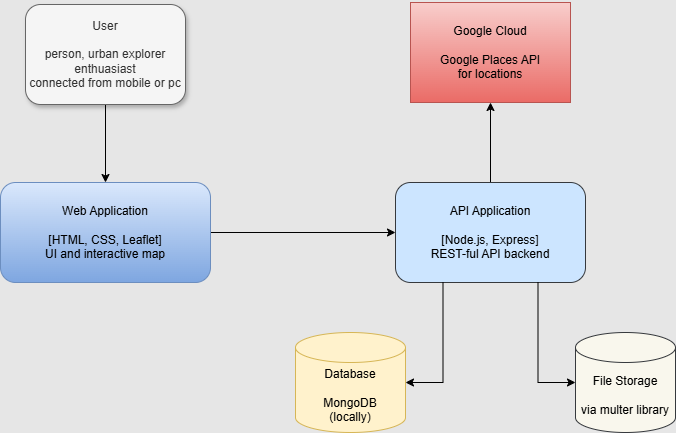
\includegraphics[width=0.8\textwidth]{images/licenta.drawio.png}
\end{center}

\subsection{Frontend Architecture}

The frontend is entirely made in html and css, with the behvaiour being indicated by javascript pieces of code. Each html page is stored in the views folder, whereas the style sheets are in the styles directory, part of the public folder, as seen from the screenshot below:

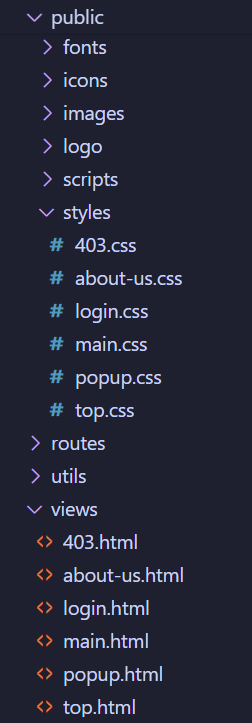
\includegraphics[width=0.15\textwidth]{images/front.png}

In public, fonts and icons are also stored in their respective folders, all of them being free for commercial use, while the images and logo are all my own.

Below is an image that shows how the main page looks like on the web client for the usual user.

\begin{center}
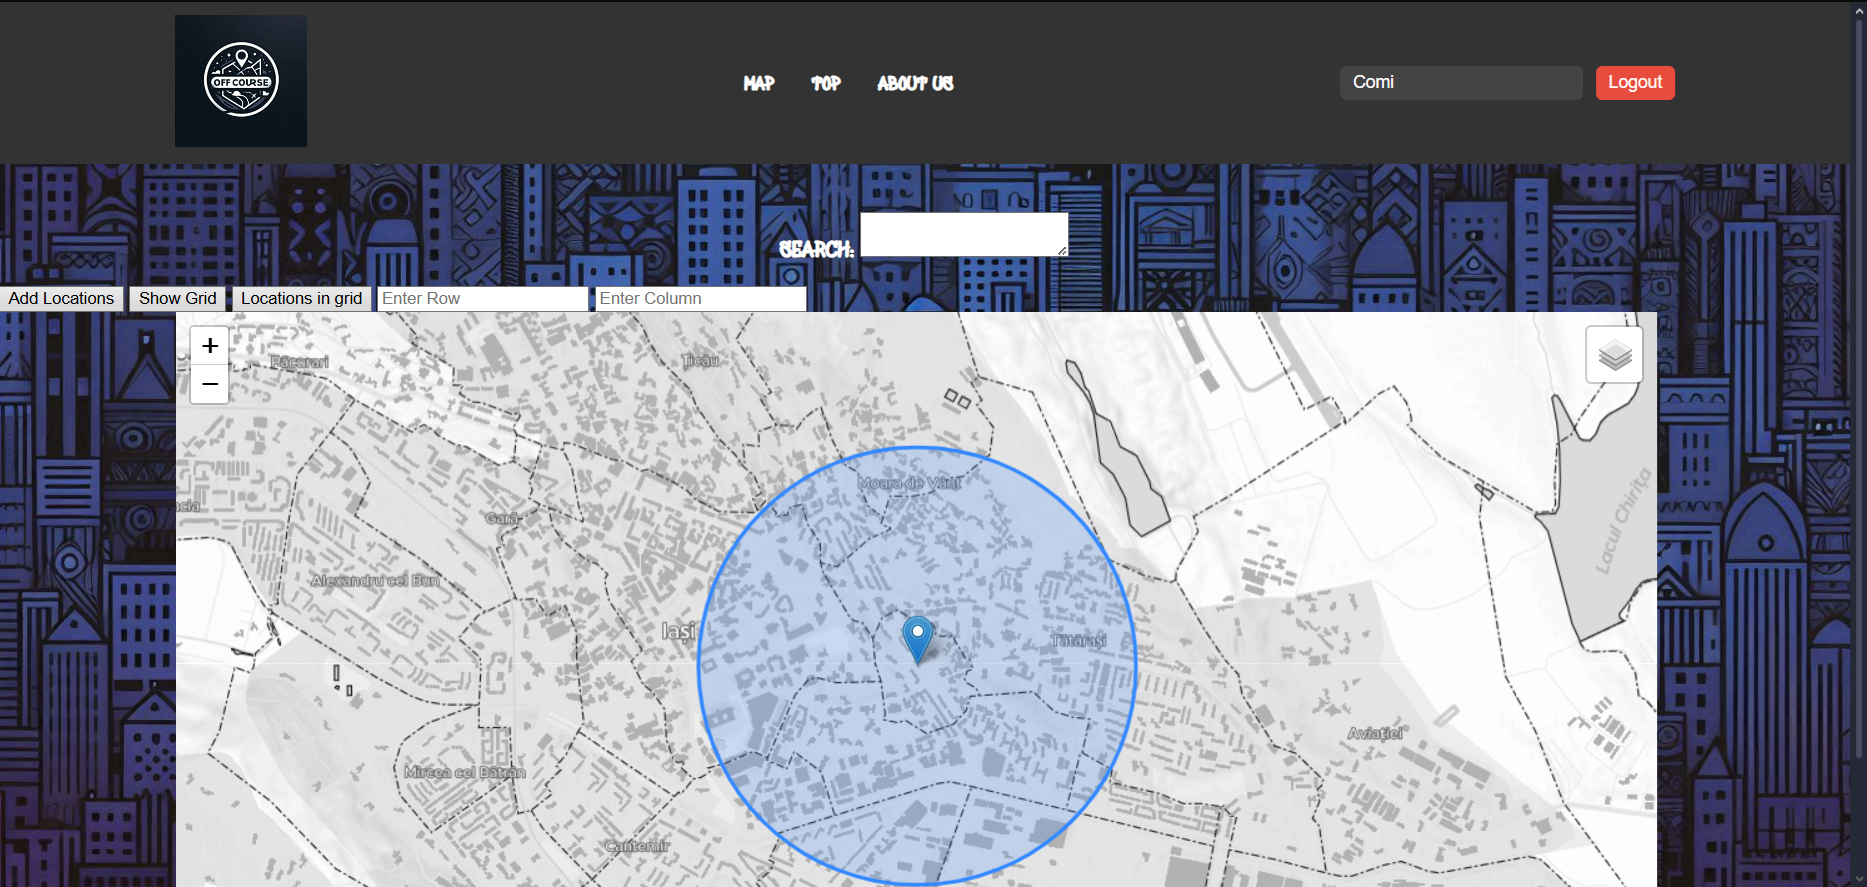
\includegraphics[width=0.8\textwidth]{images/ui.png}
\end{center}


\subsection{Backend Architecture}

As mentioned before, the project fully respects the MVC structure, having a dedicated folder for models, views and controllers, as evident from the screen capture from my code editor.

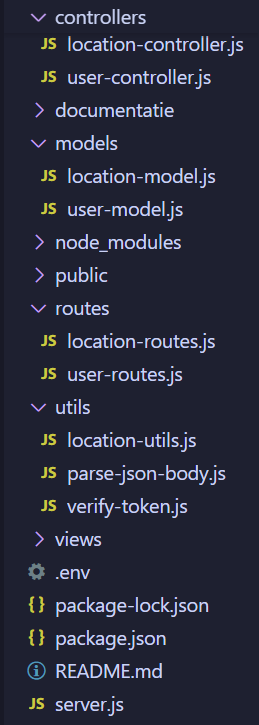
\includegraphics[width=0.15\textwidth]{images/back.png}

Other than those, there exist a folder for routes for the api, a folder with utility scripts like the one that parses a JSON file or that verifies that the cookie token is valid and, of course, the actual server.js file that starts the server, along the .env file that contains the hidden variables. 

\subsection{Database Design}

The MongoDB database is quite simple and only contains the necessary tables, those being the one that contains the users, locations, the images, the requests and the comments on locations.

\begin{center}
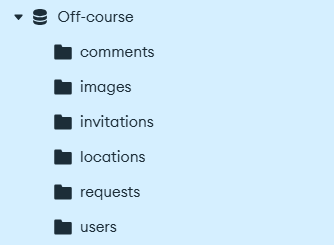
\includegraphics[width=0.6\textwidth]{images/database.png}
\end{center}

Other information that is displayed in the application is either extracted from these tables or calculated.

\chapter{Technology Stack and Implementation}
\section{Technology Selection Rationale}

All of the technologies chosen for creating this project are very popular in the industry and for good reason. Not only are they efficient, scalable, etc. but also intuitive and easy to understand for a computer science student that is not a professional in terms of creating a website.

Below I will talk about each technology in their respective sections and I will state reasons as to why I chose them.

\subsection{Frontend Technologies}
The frontend technologies were chosen for both their simplicity and also their efficiency. 

\textbf{HTML5, CSS3 and vanilla Javascript} for the user interface part of the project are enough to create a good looking website that can be accessed both easily on a computer, but also on the go, on a phone. That is why no frameworks have been used like React or Angular, since they can tank the performance of the website for some people. As well as that, I believe that a sophisticated look like the one these types of frameworks could have generated would not be enticing to the users of this application, because what is attractive for them is the concept of the platform, not the way it looks.

This is not a bad choice and is backed by the fact that some of the biggest companies in the world also went with it:"Choosing between Vanilla JS and frameworks isn't about picking a winner - it's about finding the right fit for your project. Netflix's move shows that simplicity can sometimes be the best choice."~\cite{vanillaVsFrameworks}

For mainly the same reasons, \textbf{Leaflet} has also been picked as the solution to displaying the map on the main page. It is fast by using efficient loading strategies, good for mobile, customisable in terms of look and markers and works really well with Google Maps.

"Leaflet is designed with simplicity, performance and usability in mind. It works efficiently across all major desktop and mobile platforms, can be extended with lots of plugins, has a beautiful, easy to use and well-documented API and a simple, readable source code"~\cite{leafletJs} is what the creators of the extension say about it and after using it in this project, I can personally confirm it is true.

The markers for abandoned buildings are a custom icon and there are two modes the map can be in: dark mode (default) and normal mode.

The map has all of the basic features, like a circle around the user point that indicates how accurate the actual location is, zooming in and out and scrolling on the map to anywhere in the country to view any locations and the optimisation that comes directly from the leaflet middleware.

The library that glues everything together is \textbf{Axios}. It is the one that handles communication between the client and the server in both ways. Fetch can also be used, but Axios has some clear advantages over the normal way and those are: easier communication via JSON's "A significant difference between axios and fetch is in handling JSON data. axios automatically transforms the response to JSON format under the hood, allowing you to use the response data directly const data = await response.json()"~\cite{axiosVsFetch}, custom error handling "fetch requires manual conversion of the response to JSON and does not throw errors for HTTP status codes like 400 or 500."~\cite{axiosVsFetch} and many more, for no extra cost of using this library in your project.

\subsection{Backend Technologies}

\textbf{Javascript} works really well to tie in together the frontend and backend parts: "Javascript is a flexible multi-paradigm programming language largely used in the web-development space for both front-end and back-end applications. Whereas HTML and CSS describe the elements on a webpage, code written in JavaScript makes them interactive. A framework such as NodeJS allows back-end code to be written in JavaScript."~\cite{JavaScript}

On top of the advantages mentioned above, \textbf{Node.Js}, the main framework of Javascript has a various collection of libraries that make the development significantly easier and more efficient via the npm system. Some of these packages that have also been used in this project are: jsonwebtoken, bcrypt, dotenv, cors, axios and multer.

So, \textbf{jsonwebtoken} is responsible for storing sessions on the server side, but rather in the browser client via cookies. It is secure because the cookie is always signed, so an attacker would not be able to change information about his session (like changing his level to a higher one or becoming an administrator) because he would need to know the secret signature which is hidden to all users.

\begin{center}
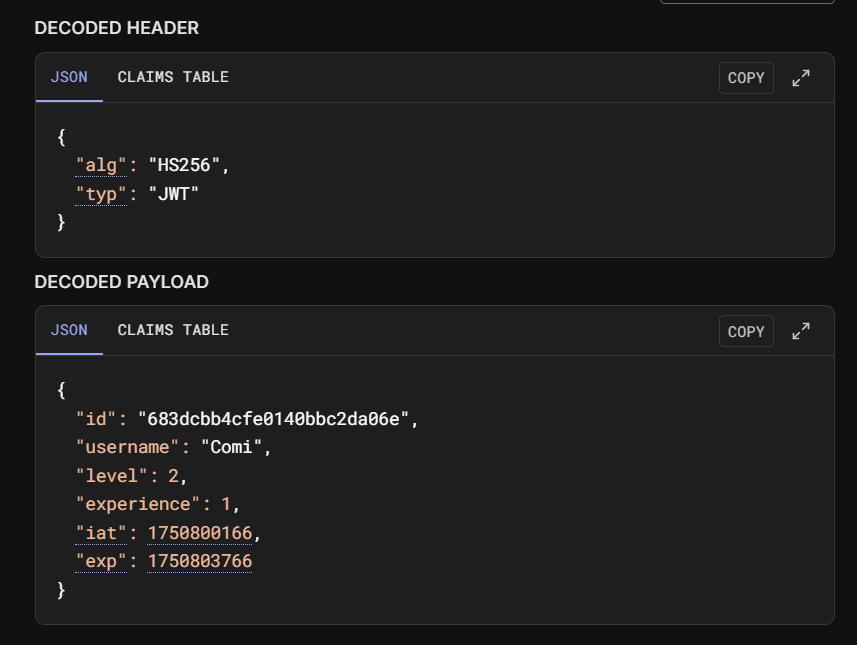
\includegraphics[width=0.6\textwidth]{images/token.png}
\end{center}

jwt.io is a website where developers can test if their cookies are working as expected in terms of data from the heads and especially the payload without extracting them in the code, which is very convinient. The signature password is obviously not available for safety reasons, but all of the relevant fields I thought necessary can be seen here, like the mongodb id, the username, the user's level and experience points and also when the token was created and when it expires.

The library used for data encryption is \textbf{bcrypt}. The 'b' in its name comes from the Blowfish cypher which is a block cipher notable for "its expensive key setup phase"~\cite{blowfishCipher}

It is expensive because after 'salting' the data, meaning it adds a string to the actual password, it is hashed a number of times, around 64 usually, which ensures that it is immune to rainbow table attacks (existing tables of hashed passwords) or brute force attacks (generating and testing out a lot of passwords), which are the most common and dangerous types of exploits when trying to get into users' accounts.

\begin{center}
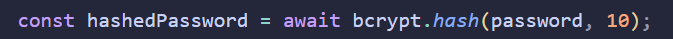
\includegraphics[width=0.7\textwidth]{images/bcrypt.png}
\end{center}

Cross-Origin Resource Sharing, or \textbf{CORS} is essential for communication between the frontend and backend in a secure way, so no other attackers from unknown addresses can interact with the server in any way. It is very easy to setup, having to just write this line of code when setting up your server: 

\begin{center}
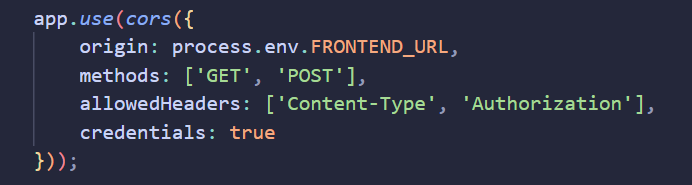
\includegraphics[width=0.6\textwidth]{images/cors.png}
\end{center}

The final but the most important file in terms of security is the \textbf{.env} file. It is used for configuration when the sever starts and it houses the private variables needed in the code for development, but that could also be used in a malicious way by attackers if they had access to their values (example: api key), so those variables are declared in that special file and their value in the backend code can be accessed via process.env.variable name.

\subsection{Database and External Services}

\textbf{MongoDB} is a database system based on JSON, not on usual SQL, which proves to be quite convienient when working with only JSON's. This makes it so communication doesn't require extra mapping and it is more efficient. As well as that, the schema is very flexible, the admin can just add or remove fields from the object's documents easily, which makes it easier to adapt to extra data that needs to be stored in terms of location (or user) data. As well as that, the connection between the server and the local database is very easy to establish, thanks to the mongoose library: "const mongoURI = 'mongodb://localhost:27017/Off-course';"

The locations that are not user submitted are extracted from the Google Maps database, using the \textbf{Google Places API} in a query like so:

\begin{lstlisting}
const url = `https://maps.googleapis.com/maps/api/place/nearbysearch/json?location=${centerLat},${centerLng}&radius=${LOCATION_RADIUS}&key=${GOOGLE_MAPS_API_KEY}`;
\end{lstlisting}

The parameters that need to be configured are the latitude and longitude coordinates, the radius and the api key provided by Google, generated in the Cloud account.

\begin{center}
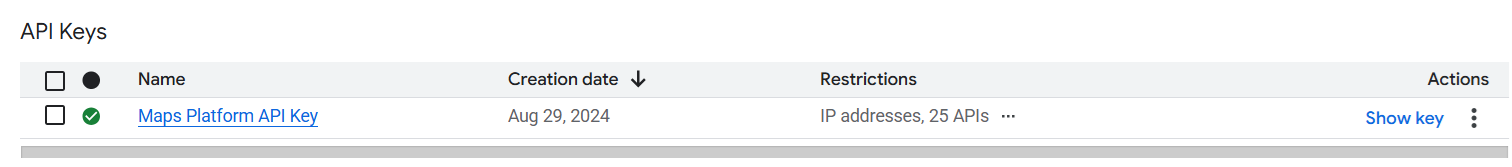
\includegraphics[width=0.8\textwidth]{images/google.png}
\end{center}

The algorithm to search for new abandoned locations works iteratively. It firstly sections a city into multiple sections, similar to red squares on the map, with each box having a row and column number, which appears when clicked on:

\begin{center}
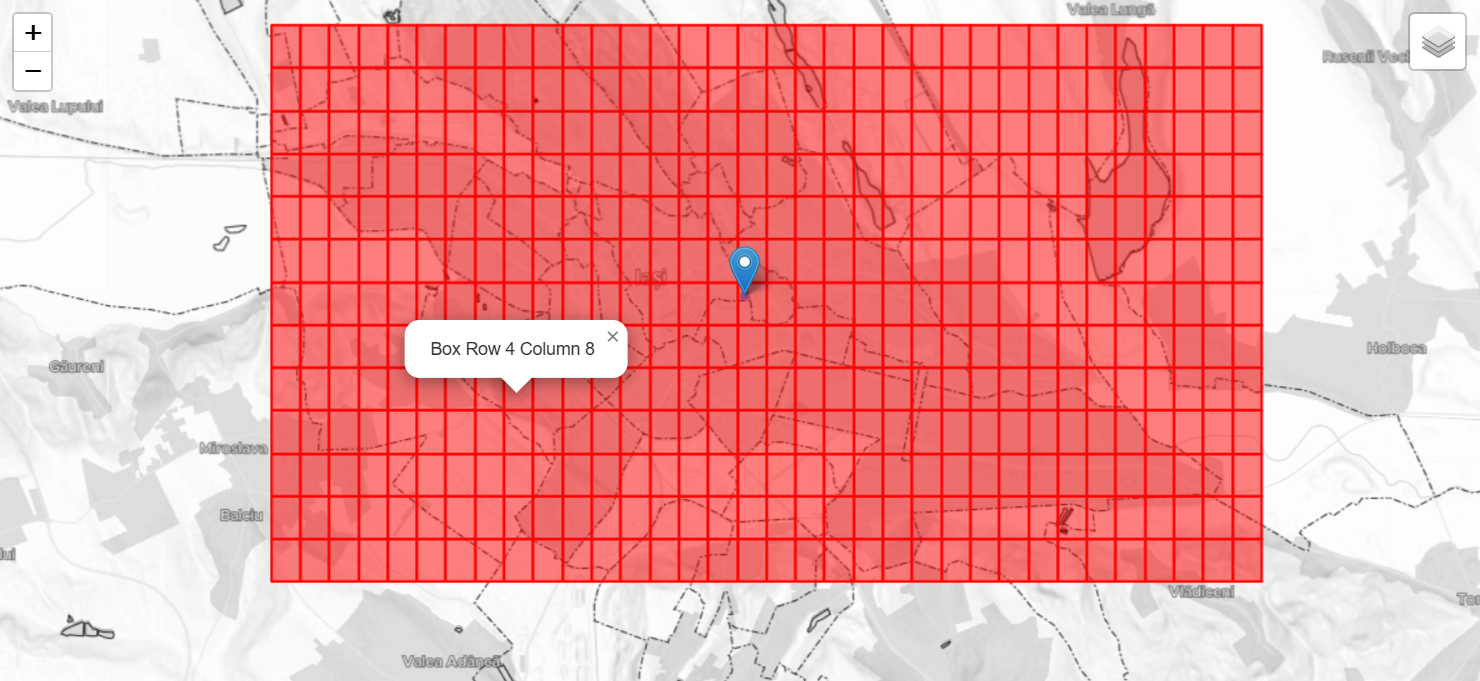
\includegraphics[width=0.6\textwidth]{images/grid.png}
\end{center}

A query or multiple queries can be done in the vicinity of that square via the radius attribute, which ensures that the whole city can be searched without overlapping quries and wasting Google Cloud credits. At maximum, 17 locations can be returned per query, and this is an example of how one such location is sent to us by google in json format:

\begin{center}
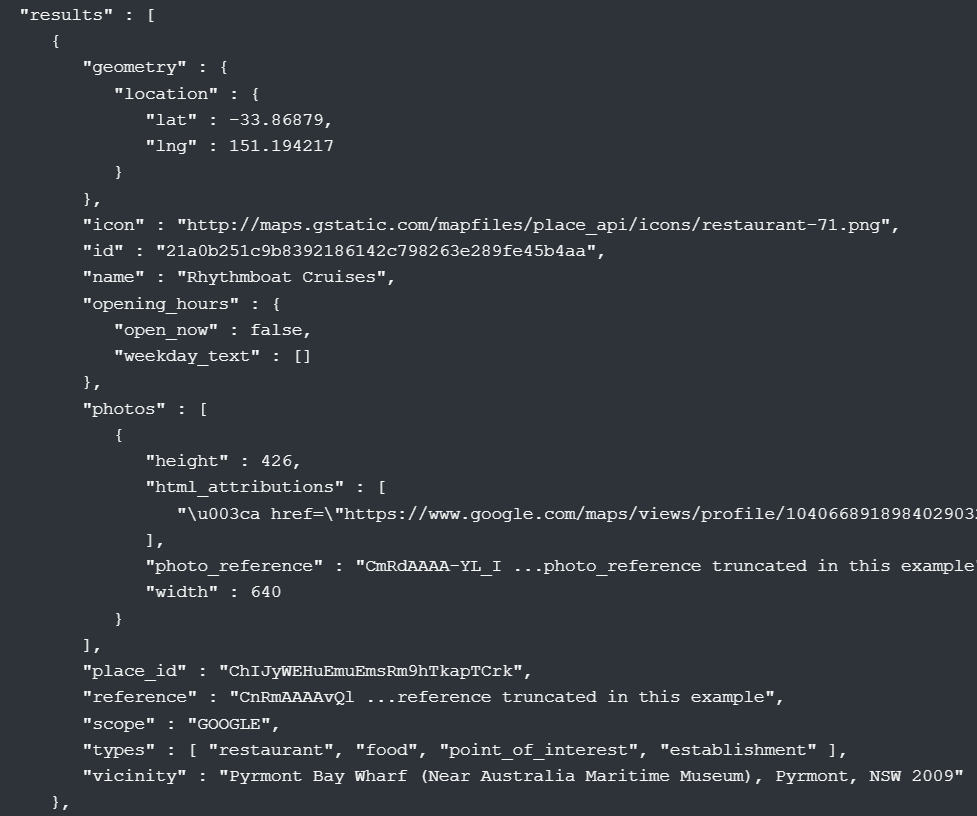
\includegraphics[width=0.7\textwidth]{images/json.png}
\end{center}

A lot of attributes are sent and more can be added or deleted, but the one that is most useful for this application is the value of business status. Abandoned buildings, obviously, will not have an active business status, rather, it will appear as CLOSED PERMANENTLY or CLOSED TEMPORARILY, instead of OPERATIONAL (these are the only 3 possible values).

The details about these closed locations are then stored in the database, with their origin attribute being set as API, meaning it has yet to be confirmed.

A great tool that was helpful with keeping track of the development process was \textbf{Github}. It's a popular solution for managing working code and it makes sure that: you are up to date when changing anything about the project, you don't accidentally delete something important and you also work in an organised environment:"Having started as a developer's collaborative platform, GitHub is now the most significant cloud-based storage space of collaborative software projects that exist on the planet."~\cite{gitHub}

It is important to know how to use this service as it is used by basically all companies and solo developers out there and it's also a great way to showcase open source code (like this project is) to the world.

The commands to push your new code to your github repository are very easy to follow after you've already created the project. From command line you have to type git add . which adds all the files to Git locally on your pc. After that you do git commit -m and then write a description of what you have worked on. And finally, you enter git push origin branchname, because it is always recommended to work on a different branch and not uploading changes directly to the main branch, as if anything is incorrect, there is no way to revert it. It is important to only push the code after you have achieved everything you set out to do on that branch and after you make sure the code is functional. After that, the application will merge your old code with your new code automatically.

\section{System Implementation}

This section will go into a bit more detail as to how the platform was implemented and how the technologies described before have been integrated.

\subsection{Database Schema Implementation}

This is the model of a location, basically how it should be stored inside the database by the server.

\begin{lstlisting}
    const locationSchema = new mongoose.Schema({
    name: String,
    latitude: Number,
    longitude: Number,
    score: {
        type: Number,
        default: 1
    },
    origin: String
});
\end{lstlisting}

Each object from the database has its own javascript model, created with the schema function from the mongoose library.

As mentioned before, data is validated before being inserted directly into the database from the backend. As well as that, protected fields like the password value is hashed beforehand.

\subsection{API Endpoints Design}

The \textbf{REST-ful API} uses HTTP requests, mainly GET and POST for communication with JSON bodies. The endpoints are declared in the server.js file as seen below.

\begin{center}
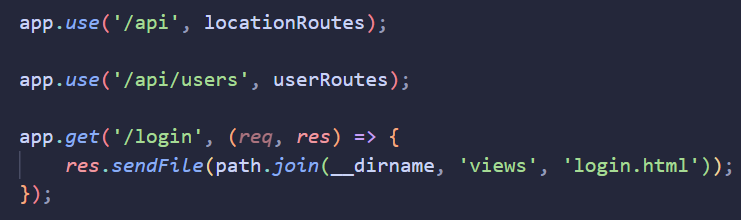
\includegraphics[width=0.8\textwidth]{images/api.png}
\end{center}

There is a specific api endpoint for the pages, the locations, the users, etc.

Each endpoint has explicit error handling and also status codes for requests, so in case of something going wrong, the reason will be clear from the console logs.

\subsection{Authentication Implementation}

The \textbf{verify-token.js} script is responsible for making sure users are logged in and can access pages, by checking wether or not the cookie token created when a user logs in or signs in is valid.

\begin{center}
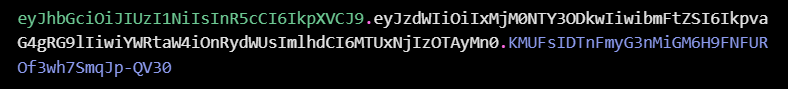
\includegraphics[width=0.8\textwidth]{images/signature.png}
\end{center}

The crucial part is the third one, the one in blue, as that represents the signature of the cookie that dictates to the server wether or not it was created by it or someone else (like an attacker).

The screenshot is taken from JWT.io where cookie headers and payloads can be decrypted to check if they are correct or not.

If the token appears to be incorrect, the user is redirected to the /403 page, being told that he has no access and should sign in or log in. He will not be able to view any other information from the website.

\subsection{File Upload Implementation}

After an explorer submits a form for a location and includes a photo, with the help of the multer npm library, the image will get stored in the database for the future.

"Multer is a node.js middleware for handling multipart/form-data, which is primarily used for uploading files. Multer adds a body object and a file or files object to the request object. The body object contains the values of the text fields of the form, the file or files object contains the files uploaded via the form."~\cite{multer}


\chapter{Testing and Validation}
\section{Testing Strategy}

The testing that was done for the platform was more so practical rather than with automated validation like unit tests. This is because the target audience of the project is a relatively small community and the testing was made to reflect their behaviour using the website.

\subsection{Functional Testing}

All of the experimentations to figure out wether or not Off Course is usable, intuitive and safe was carried on by me personally and a friend of mine that is also part of the urbex community.

These are the points that have been tested:

\begin{enumerate}
    \item user registration, logging in and out
    \item locations submission and viewing
    \item uploading photos and descriptions
    \item gamification features like gaining experience and leveling up
    \item mobile experience
\end{enumerate}

\section{Performance Results}

In order to quickly and easily see how well the website performs without any intricate tests is a Chrome extension that automatically analyses the efficiency and lets you know how well it performs and where to improve:"You can run Lighthouse as part of PageSpeed Insights, in Chrome DevTools, from the command line, or as a Node module. You give Lighthouse a URL to audit, it runs a series of audits against the page, and then it generates a report on how well the page did."~\cite{lighthouseChrome}

\begin{center}
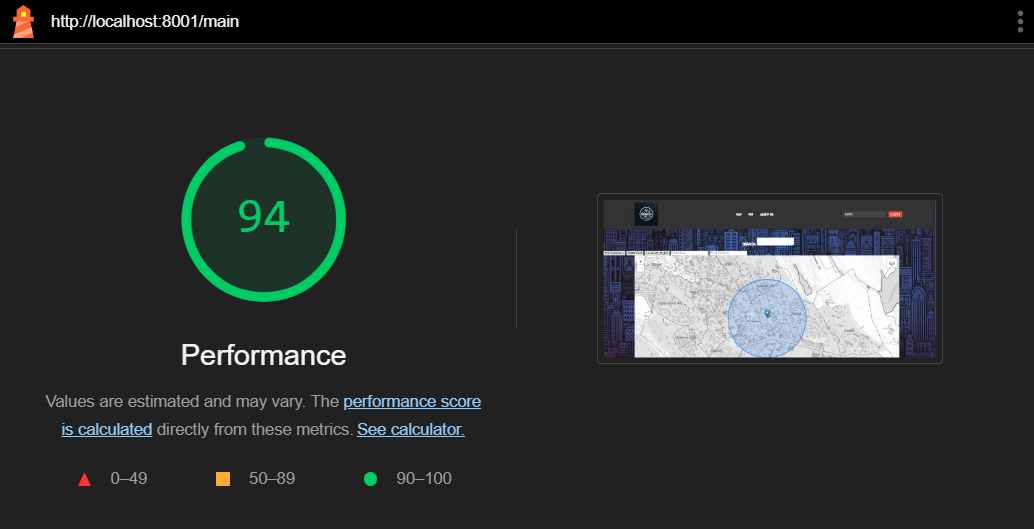
\includegraphics[width=0.7\textwidth]{images/lighthouse.png}
\end{center}

As seen from the screenshot above, the website has a high 94 percent performance with very few aspects to improve on in terms of efficiency. It performs well for both desktop and mobile with very fast load times that are definitely industry standard. So the technologies chosen seem to have been correct, as the site works well, though some changes can be made for an even better flow in terms of loading pictures with multer and more efficient caching.

\section{User Feedback}

The feedback from my friend was positive in terms of looks, the leveling and leaderboard features and mobile experience. It is important to note that after the application is published, changes can be made according to users' suggestions and improvements. Nothing is final.

\chapter{Deployment and Hosting}
\section{Hosting Solution}

Hosting for the application will happen locally, not in the cloud. The main reason for choosing this approach is because by not relying on Cloud services like Amazon, Microsoft or other lesser known ones, even though they are mostly trustworthy and efficient. The main problem with these is the subscription-like fee you have to pay in order to keep the server running and also not owning the domain you actually host your website to. In terms of scalability and performance, the two options are more or less the same.

*Side note: While at the Faculty of Computer Science, I have deployed multiple projects to the cloud, namely Microsoft Azure, but never have I hosted an app on a raspberry pi, this new experience being a learning point for me personally.

\subsection{Raspberry Pi Deployment}
The Raspberry Pi is a small computer that can be used to 
"Whatever your application and whatever your scale, Raspberry Pi offers cost effective, high performance computing for businesses and the home."~\cite{raspberryPi}

\begin{center}
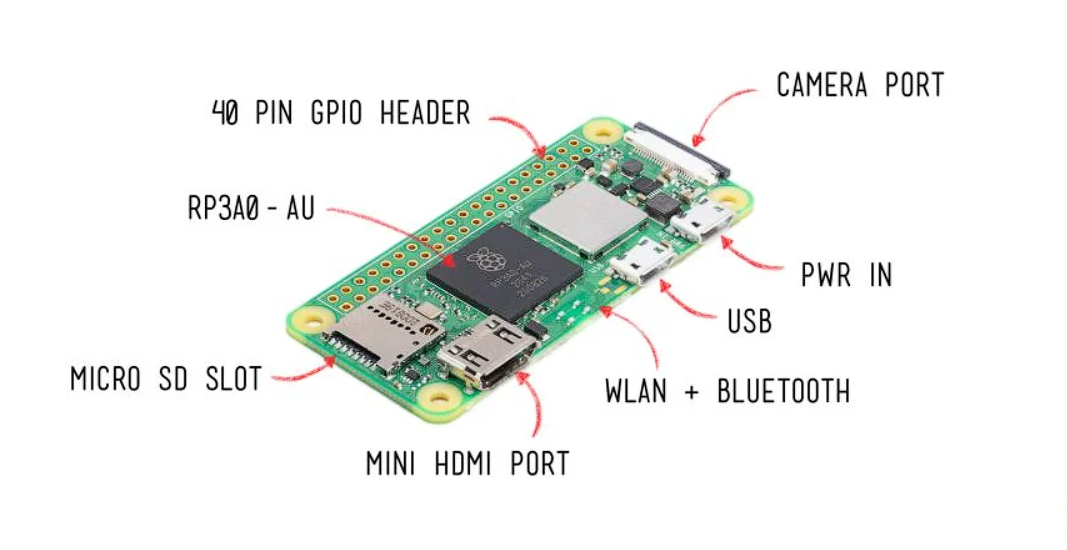
\includegraphics[width=0.8\textwidth]{images/raspberrypi.png}
\end{center}

The \textbf{Raspberry Pi Zero 2 W} model is very cost effective, being less than 100 RON online, while at the same time having the following specifications:

\begin{itemize}
    \item 512MB RAM
    \item 32GB MicroSD
    \item ARM Cortex-A53 quad-core processor at 1GHz
    \item Wi-Fi connectivity for internet access
    \item 5W power consumption
\end{itemize}

These specs are more than enough to host a dedicated web applicaiton, especially with the low traffic Off Course expects because of the exclusivity of the users.

The way of setting up the mini computer to run a server is not difficult, the process being simplified by nginx, the proxy service that allows hosting to be created on a router at home "Nginx (pronounced "engine x") is a web server that can also be used as a reverse proxy, load balancer, mail proxy and HTTP cache. As of April 2025, W3Tech's web server count of all web sites ranked Nginx first with 33.8 percent."~\cite{nginX}

Other than that, though, the rest of the process is quite straight forward, just having to set up Node.js, MongoDB and the source code on the Raspberry Pi in order to host it.

\subsection{Domain and DNS Configuration}

A .ro domain (offcourse.ro) has been registered for Off Course on the official Domain Registry of Romania - \textbf{ROTLD}. "RoTLD este autoritatea oficială (registru) pentru domeniile .ro. Asigurăm că fiecare domeniu .ro este disponibil, din punct de vedere tehnic și că acesta este înregistrat o singură dată la nivel mondial."~\cite{roTLD}

\begin{center}
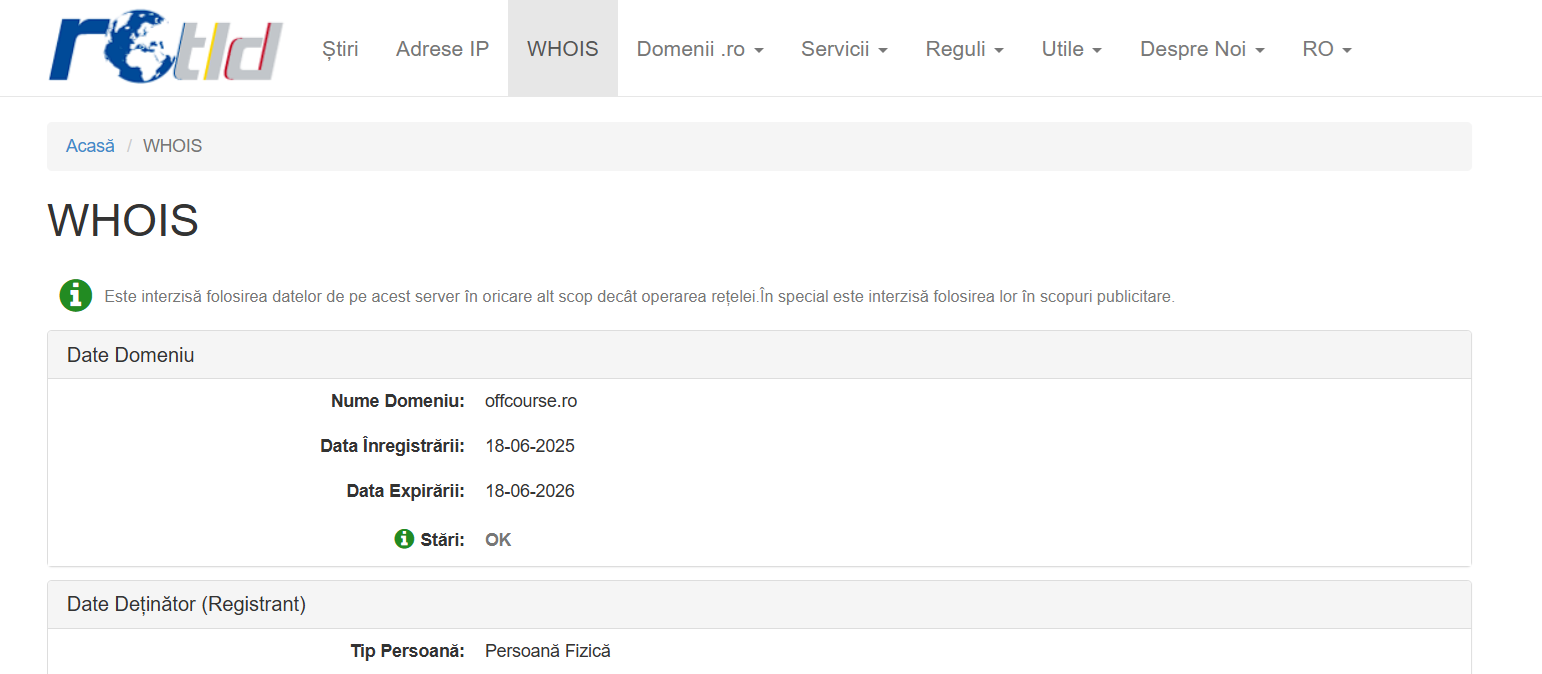
\includegraphics[width=0.8\textwidth]{images/dns.png}
\end{center}

The main issue that comes with using a wifi router provided by an Internet Service Provider is that the external IP address it has changes all the time. One way to counter this is to use a service like noip.com. 

What it does is it monitors the IP address of the router and when it changes, it will update it on the DNS. This creates the same behaviour as a static IP address that is needed for having the website up indefinitely. The best part about it is that a user of their platform can register one hostname for free: "This will allow you to run your servers or check your devices remotely at your home or business without a static IP address."~\cite{noipDNS}

\section{Production and Maintenance}

After having the website up and running, there are a couple of ways to check wether or not it is running correctly. 

Nginx has a feature that tracks usage patterns in their logs. MongoDB can monitor the database performance and, of course, custom loggings from the server can keep track of internal operations.

As the application grows and after looking at these metrics, it can be determined wether or not improvements can be made in terms of refactoring or rewriting code to optimise it or maybe switching to a cloud-based hosting system.

\chapter*{Conclusions}
\addcontentsline{toc}{chapter}{Conclusions}

\section*{Main Contributions}

In terms of technology, I successfully created an algorithm that can extract closed locations from the Google Maps database. Filtering or querying by this specific attribute is not possible otherwise. The way of doing it is not efficient and can be costly in terms of requests, but no other better way is possible.

From the social aspect point of view, a new and unique plaform for urban exploring enthusiasts in Romania now exists. The application centralises all the existing data and brings new data from Google, it has quality control over the people that are allowed to join it and has a gamification system that can bring a fresh and fun feeling to this hobby.

\section*{Objectives Achievement Analysis}

All of the objectives mentioned in the first section have been achieved successfully. 

Off Course is a working modern website that has a collection of abandoned locations from Romania, displaying them on a map for all users that are invited. The data is displayed on a map. Users have a lot of features available to them and also using the app is secure, efficient and intuitive.

\section*{Lessons Learned}

On a personal level, by working on this project I was reminded how to develop a website using HTML, Node.Js and a database such as MongoDB, qualities I learnt during university. On top of that, it was a great learning experience for new things I have never tried before, like using the Google Cloud for API, implementing a working map, setting up a domain and hosting a server on a raspberry pi, locally and many more.

I learnt a lot more things than those on the technical side, like how to research solutions in order to solve a problem that clearly exists in a community, to listen to feedback by test users or future users of the platform and how to manage my time in order to develop such a big project over the course of weeks, while still attending classes at the faculty and going to an internship.

I am sure that all of the lessons I have learned from using these frameworks, cloud services, libraries, type of database and pieces of hardware needed to host the project will help me in my work in the future.

\section*{Future Work and Improvements}

Speaking on the future, this is a project that I was really passionate about creating and really excited to use, now that it is complete. Updates to improve the application will definitely be made, these being also in terms of what I think would be best moving forward from my own point of view, but also from what the users will say about it.

In the coming months, other than trying to complete the dataset of abandoned locations in the country, a taks which seems almost impossible, I also want to add features to the website, those being mainly improvements that will help in the social aspect, like uploading videos, a friendship system that will also allow you to tag other users and so, gain experience together. But I would also like to improve on the technical side, with a better looking UI and an integration with Instagram (which is the main platform urban explorers also share their work). In the case that it is required for scalability, I would also be open to porting Off Course on the cloud, but for now, I can say I am content with its state and will let the future speak in terms of these measures.

Closing words: Off Course is not only just a web application designed to better my abilities as a programmer and prove my worth after finishing the Faculty of Computer Science. It's a passion project created with much determination and implication for the Urban Exploring community that exists in Romania and needed a solution like this modern, intuitive, responsive, powerful and efficient platform that promotes the preservation of old, forgotten locations and the responsibility of the users in its fanbase. I am proud of this project and I am happy to share it with the world.

\bibliographystyle{IEEEtran}
\bibliography{references}

\end{document}